% =====================================================================================
% SECTION 3: DESIGN AND IMPLEMENTATION
% =====================================================================================

\section{Design and Implementation}
\label{sec:design}

\subsection{System Architecture}
\label{subsec:architecture}

Our solution uses a modular web-based architecture with four main components:

\textbf{Data Processing Layer:} Handles CSV file loading, time calculations, and event filtering using pandas and pm4py libraries. This layer ensures data integrity and performs the required time since case start calculations.

\textbf{Visualization Engine:} Built with Dash and Plotly, generates interactive violin charts with real-time updates. The engine supports dynamic plot generation and handles user interactions for sorting and transformation changes.

\textbf{Transformation Module:} Implements seven different time scaling methods to handle various distribution characteristics. Users can switch between transformations to reveal different aspects of the timing patterns.

\textbf{User Interface:} Responsive web dashboard with sidebar controls for dataset selection, transformation options, sorting parameters, and event count configuration. The interface provides immediate feedback for all user actions.

The modular design ensures maintainability and allows easy extension with new datasets or transformation methods.

\subsection{Event Filtering Algorithm}
\label{subsec:filtering}

The core innovation is our filtering approach that solves the case-start event problem. The algorithm works as follows:

\begin{enumerate}
    \item Load event log data from CSV file
    \item Calculate time since case start for each event
    \item Filter out events where time since case start equals zero
    \item Count event frequencies and select top N most frequent events
    \item Validate data integrity and return filtered dataset
\end{enumerate}

This simple approach removes 2.6-28.6\% of uninformative events across our test datasets while preserving all meaningful timing information.

\subsection{Time Transformation Methods}
\label{subsec:transformations}

We implemented seven transformation methods to handle different data characteristics:

\textbf{Logarithmic:} Uses log(hours + 1) for highly skewed data with extreme outliers. Most effective for Traffic Fines and BPI datasets with long time ranges.

\textbf{Raw Time Units:} Preserves absolute timing in hours, days, weeks, or months. Best for time-critical processes like healthcare where absolute timing matters.

\textbf{Square Root:} Provides moderate compression using sqrt(hours). Good middle ground for business processes with moderate skewness.

\textbf{Min-Max Scaling:} Normalizes data to 0-1 range for cross-dataset comparison. Enables comparing timing patterns across different process domains.

Each transformation reveals different aspects of the timing patterns, giving users multiple perspectives on the same data.

\subsection{Violin Chart Implementation}
\label{subsec:violin_charts}

Our violin charts combine the strengths of multiple visualization types:

\textbf{Distribution Shape:} Shows the full distribution using kernel density estimation, revealing multimodal patterns and outliers that histograms miss.

\textbf{Statistical Summaries:} Integrated box plots display median, quartiles, and outliers alongside the distribution shape.

\textbf{Horizontal Orientation:} Accommodates long event type names while maintaining readability.

\textbf{Interactive Elements:} Users can hover for detailed statistics and click to highlight specific event types.

The implementation uses Plotly's violin chart with custom styling for optimal readability and academic presentation.

\subsection{Statistical Sorting System}
\label{subsec:sorting}

Users can sort event types by seven different statistical parameters:

\begin{itemize}
    \item \textbf{Frequency:} Total event count (default sorting)
    \item \textbf{Mean:} Average time since case start
    \item \textbf{Median:} Middle value of the distribution
    \item \textbf{Minimum:} Earliest occurrence time
    \item \textbf{Maximum:} Latest occurrence time
    \item \textbf{Q1:} 25th percentile value
    \item \textbf{Q3:} 75th percentile value
\end{itemize}

Each sorting option reveals different insights. Frequency sorting shows the most common events, while mean sorting reveals which events typically happen early or late in processes.

\subsection{Dashboard Interface}
\label{subsec:interface}

Figure \ref{fig:dashboard_interface} shows the complete dashboard interface with all interactive elements.

\begin{figure}[H]
\centering
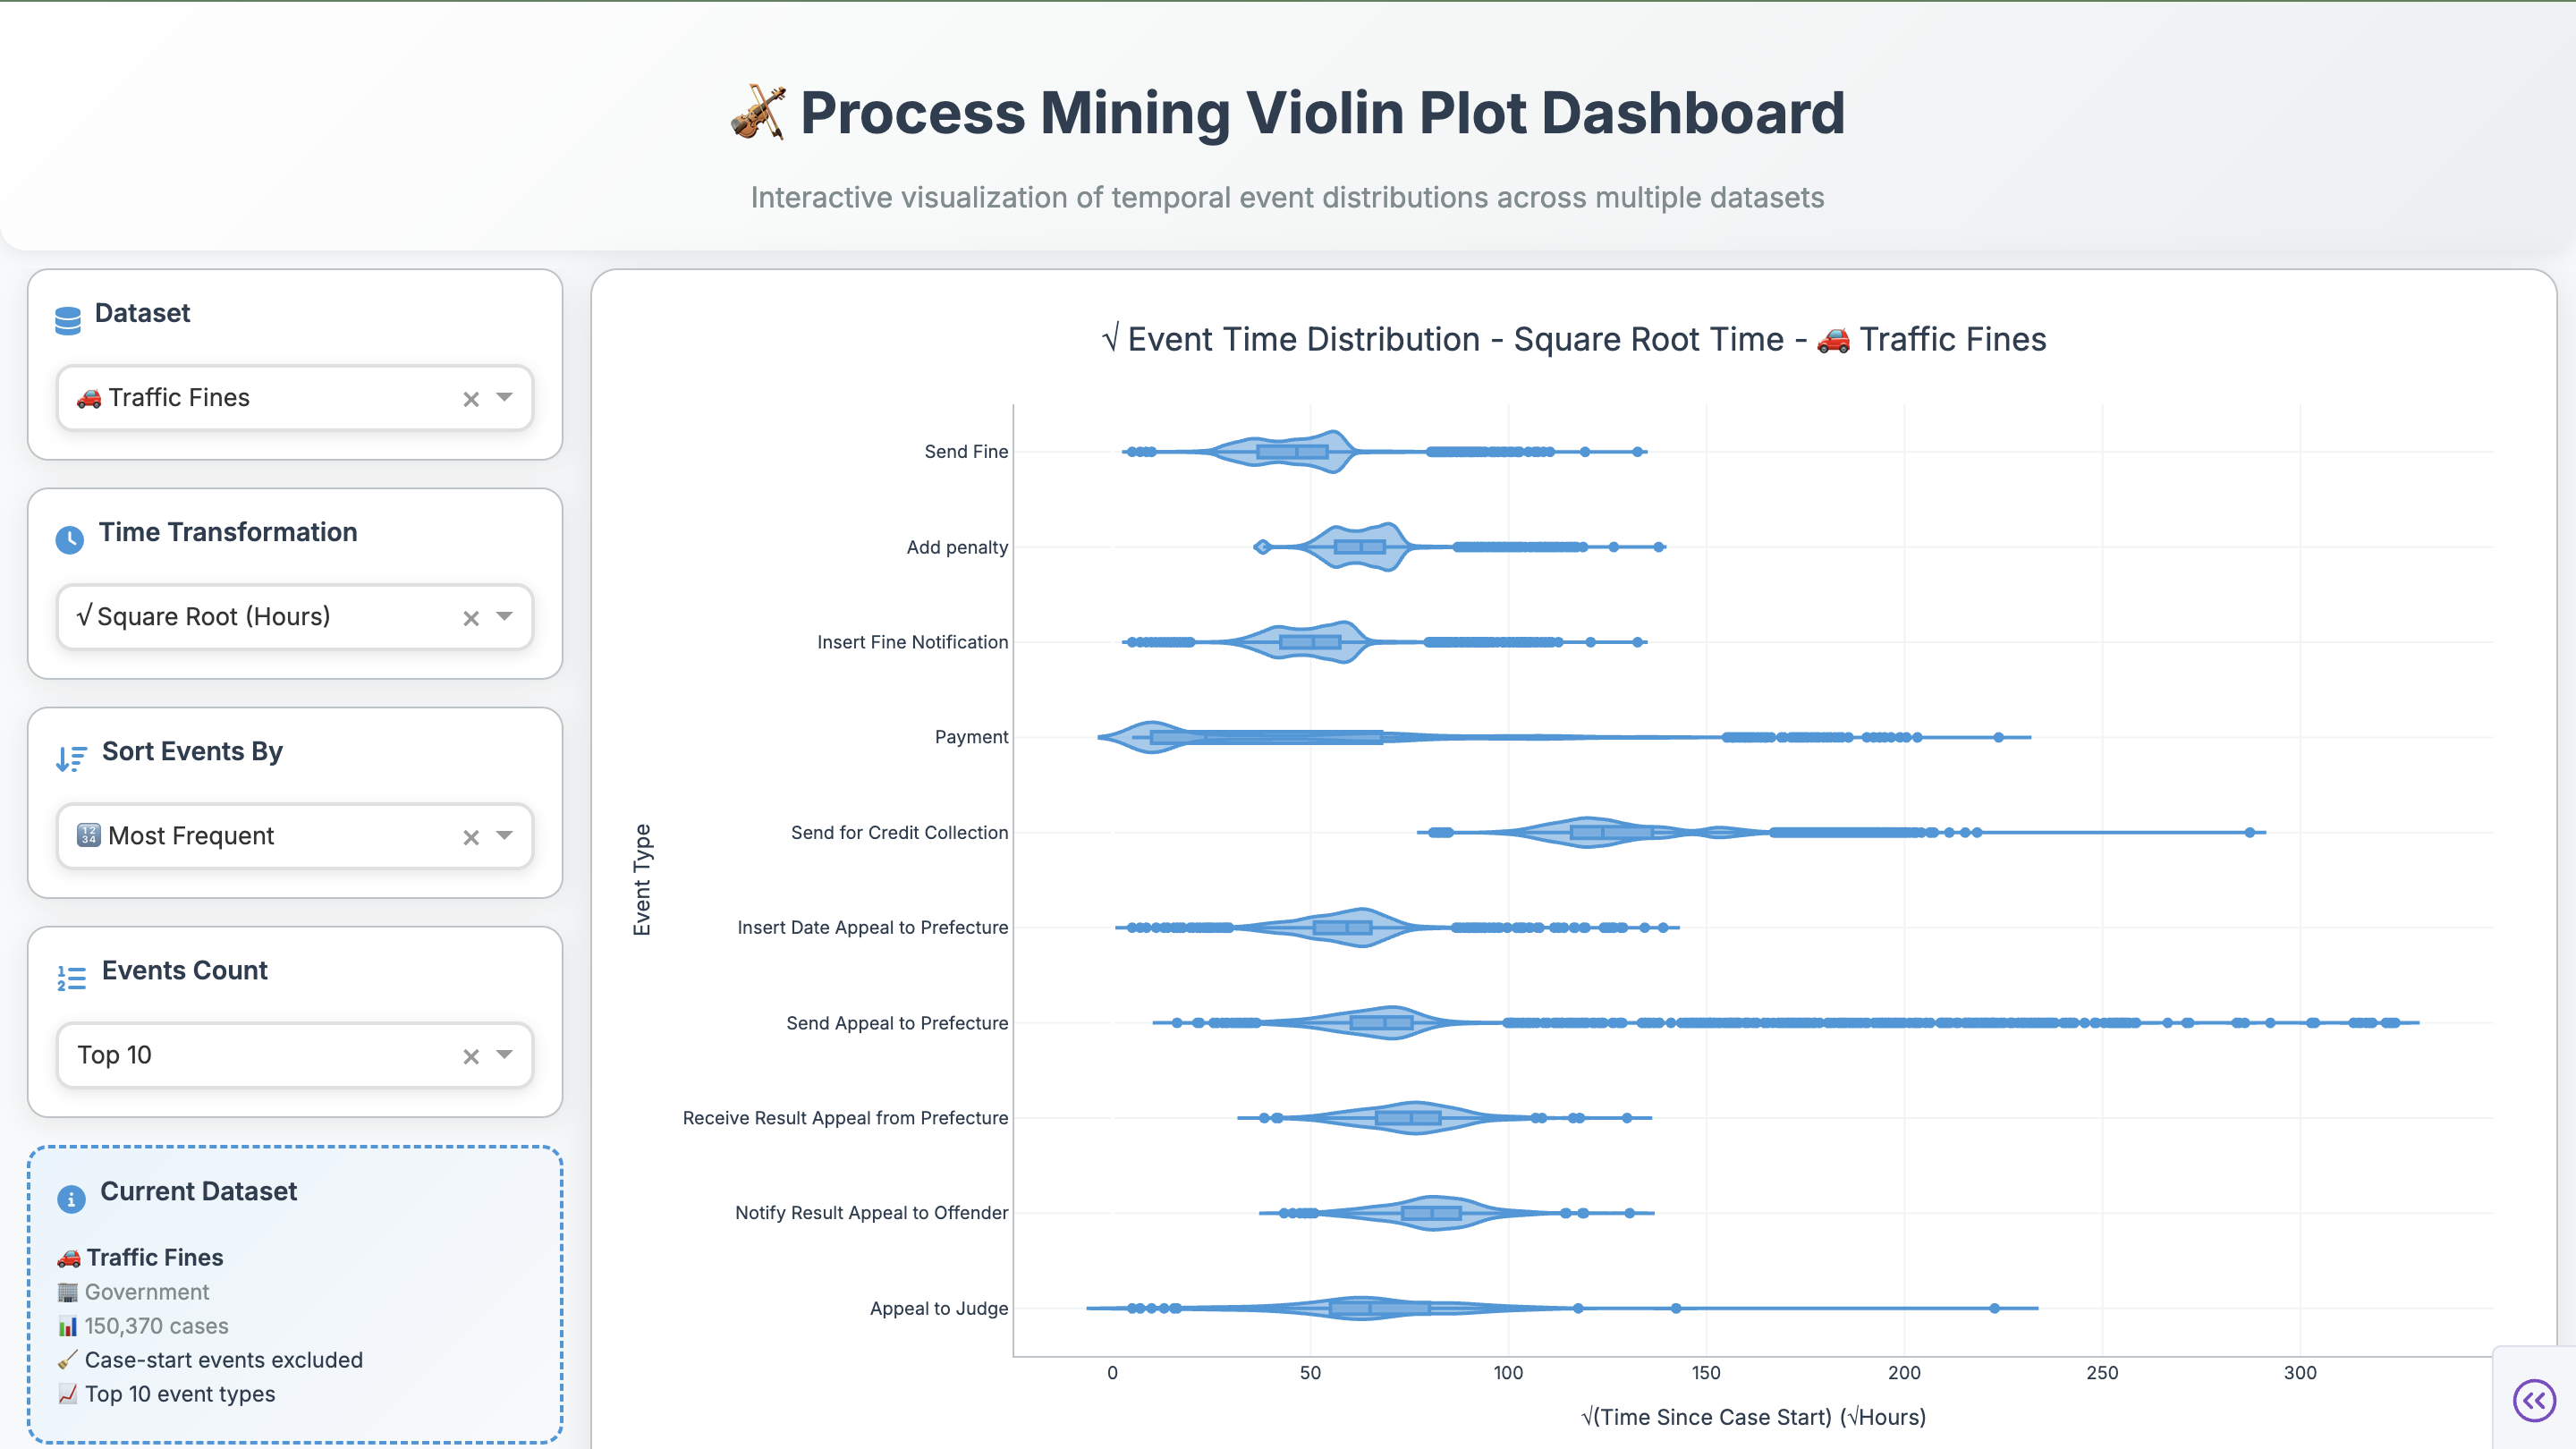
\includegraphics[width=\textwidth]{fig/dashboard_interface.png}
\caption{Complete dashboard interface showing sidebar controls and violin chart visualization. Users can select datasets, change transformations, adjust sorting parameters, and control the number of displayed events. The violin charts update in real-time based on user selections.}
\label{fig:dashboard_interface}
\end{figure}

The sidebar contains all user controls:

\textbf{Dataset Selector:} Dropdown menu for switching between Traffic Fines, BPI 2012, BPI 2017, and Sepsis datasets.

\textbf{Transformation Controls:} Dropdown for selecting time scaling methods with immediate visualization updates.

\textbf{Sorting Options:} Dropdown for statistical parameter selection that reorders the violin charts instantly.

\textbf{Event Count Slider:} Allows users to display between 4-10 most frequent events to avoid visual clutter.

\textbf{Dataset Information Panel:} Shows current dataset statistics including total events, filtered events, and filtering percentage.

\subsection{Performance Optimizations}
\label{subsec:performance}

Several optimizations ensure fast response times:

\textbf{Data Caching:} Processed datasets are cached in memory to avoid repeated file loading and filtering operations.

\textbf{Efficient Filtering:} pandas operations minimize memory usage and processing time for large datasets.

\textbf{Progressive Loading:} Only the selected number of events are processed for visualization, reducing computational overhead.

\textbf{Client-Side Updates:} UI state changes use client-side callbacks where possible to minimize server round trips.

These optimizations maintain sub-second response times even for datasets with over one million events.
